%!TEX root = ../Thesis.tex
\section{Multichannel-System in der Cloud (An-Nam Pham)}
Das Unternehmen Stylez betreibt ein Multichannel-Retailing (Mehrgleisiger Vertrieb des Handels). Wie in der Grafik \ref{img:Cloud_Implementierung} auf Seite \pageref{img:Cloud_Implementierung} zu sehen, kann der Kunde sowohl in der Filiale, als auch online per Webshop einkaufen. Gekaufte Waren können bei Bedarf ebenfalls sowohl in einer Filiale als auch online umgetauscht oder zurückgegeben werden (beim Online-Weg: Rücksendung per Post).

Die Aufgabe diese Prozesse zu steuern und zu überwachen, ist ohne Unterstützung von passender IT-Systeme kaum zu bewältigen.\\
Die Lösung für die große Multichannel-Herausforderung lautet Multichannel-System.\\
\\
Das Multichannel-System ist ein Verbund von mehreren Systemen, die dem Unternehmen dabei unterstützen, sämtliche Geschäftsprozesse und das Kundenmangement zu steuern.\\
\\
Im Kapitel \ref{sec:IT-Infrastruktur} wurden die Vorteile für einen Umzug in die Cloud erläutert.
Deswegen soll das Multichannel-System in der Cloud betrieben werden.
Die zentrale Datenbank ist die Datenbasis für das Multichannel-System. Da hier nicht nur Unternehmensdaten, sondern auch vertrauliche Kundendaten gespeichert werden, soll diese Datenbank nicht in die Cloud ausgelagert werden, sondern weiterhin vom Unternehmen betrieben werden.

Dies macht das Ganze zu einer hybriden Cloud, die aus der Private Cloud (zentrale Datenbank) und der Public Cloud besteht.\\
\\
Die folgende Abbildung zeigt die empfohlene Implementierung des Multichannel-Systems in der Hybrid Cloud:
\begin{figure}[H]
\centering
\begin{minipage}[t]{0.8\textwidth}
\fbox{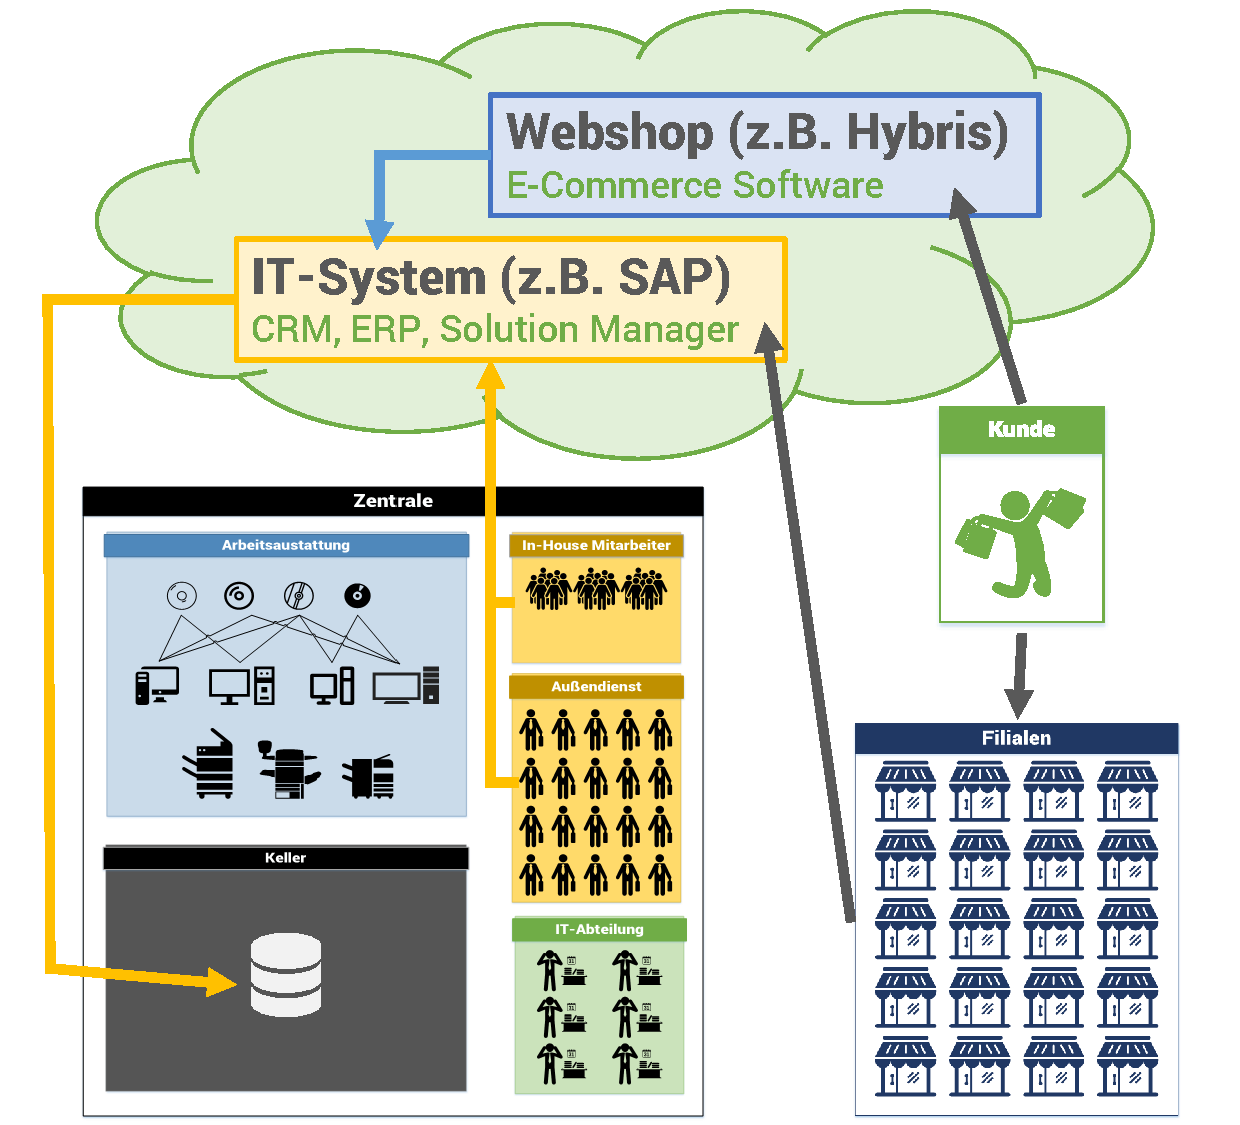
\includegraphics[width=1\textwidth]{img/Cloudinhalt.pdf}}
\caption{Empfohlene Implementierung der Hybrid Cloud} % Überschrift
\source{Eigene Darstellung} % Quelle
\label{img:Cloud_Implementierung}
\end{minipage}
\end{figure}
In den folgenden Unterkapiteln werden die einzelnen Komponenten des Multichannel-Systems kurz beschrieben und ihr Nutzen für das Unternehmen erläutert.
\subsection{SAP IT-System}
Wir empfehlen die gesamte Unternehmensstruktur von Stylez mit Hilfe von SAP im IT-System abzubilden\footnote{Berechtigungskonzept, Organisationsmanagement, Geschäftsprozesse, etc. werden in SAP ERP abgebildet, um ein optimales Business-IT-Alignment zu ermöglichen.}. Der Entscheidung für SAP bietet unter anderem folgende Vorteile\footcite[Online im Internet.]{SAP_Vorteil}:
\begin{itemize}
\item Internationaler Anbieter
\item führende Technologie
\item 40 Jahre Erfahrung mit kfm. Software
\item technische Innovationskraft
\item finanzielle Stabilität
\end{itemize}
Außerdem gibt es viele SAP-Partner, die auf den Fashion-Handel spezialisiert sind. Diese haben unter anderem folgende Stärken:
\begin{itemize}
\item Kundennähe
\item Mittelstandsausrichtung und -erfahrung
\item Angebot als Generalunternehmer
\end{itemize}
Das SAP System soll aus ein \acrshort{ERP}-System, \acrshort{CRM}-System und einen Solution Manager bestehen.
\subsubsection{SAP ERP}
Das \acrlong{ERP}-System (ERP-System) bildet (im Idealfall) das Unternehmen in seiner Gesamtheit zeitnah ab. Dadurch ist es ein sehr wertvolles Hilfsmittel für Planungs- und Steuerungsaufgaben, das unter anderem noch folgende Vorteile bietet:
\begin{itemize}
\item Erhöhte Automatisierung für kürzere Bearbeitungszeiten und Kostenersparnisse
\item Verringerte Durchlaufzeiten von Prozessen
\item Erhöhte Datenqualität, Redundanzen und Inkonsistenzen werden vermieden
\item Verbesserte Zusammenarbeit über Abteilungsgrenzen hinweg
\item Optimierter Informationsfluss im Unternehmen
\item Überwinden organisatorischer und technischer Schnittstellen
\end{itemize}
\underline{\textbf{Der große Nutzen:}}\\
ERP-Systeme tragen langfristig zur Leistungssteigerung und Kostenreduzierung bei, da das ERP-System sämtliche Bereiche wie z.B. Materialwirtschaft, Finanz- und Rechnungswesen, Personalwirtschaft, Verkauf, Marketing und Forschung abbildet. Dadurch können alle Bereiche miteinander kommunizieren und dieselbe Datenbasis nutzen. Dies spart z.B. im Vergleich zur \glqq Zettelwirtschaft\grqq~und Excel viel Zeit und Kosten.\footcite[vgl.][Online im Internet.]{ERP}
\subsubsection{SAP CRM}
\glqq Der Kunde ist König\grqq. Dieser bekannte Satz drückt ganz gut aus, worauf man in einem Unternehmen ganz besonders achten muss.\\
Das \acrlong{CRM} (CRM) (zu Deutsch: Kundenbeziehungsmanagement) unterstützt das Unternehmen dabei, die Beziehung zu bestehenden und potenziellen Kunden zu verwalten und zu gestalten.\\
\\
\underline{\textbf{Der große Nutzen:}}\\
Das CRM-System verwaltet nicht nur bestehende und potenzielle Kunden des Unternehmens. Wird das Supply-Chain-Management eingebunden, kann das CRM-System auch Lieferanten verwalten. Im Fall von Stylez können auch alle Franchisenehmer eingebunden werden.\\
Das Besondere am CRM-System ist, dass es die Historie der Kundeninteraktion verfolgbar macht. Es kann sehr schnell ein Überblick über einen Kunden, Lieferanten oder Franchisenehmer\footnote{Zur Vereinfachung werden Kunden, Lieferanten oder Franchisenehmer im Folgenden mit Kunde zusammengefasst.} geschaffen werden (z.B. getätigte Anrufe, Häufigkeit der Support-Anfragen, Anteil am Geschäftsumsatz, uvm.).
Dadurch kann schnell auf den Kunden eingegangen. Dies spart Zeit und fördert die Professionalität und somit auch das Vertrauen der Kunden. Außerdem kann das CRM-Systen benutzt werden, um Prognosen über zu erwartende Ergebnisse einfacher und genauer zu erstellen. Und es bietet volle Transparenz und bei Bedarf jederzeit Zugriff auf Kundeninformationen.\footcite[vgl.][Online im Internet.]{CRM}

\subsubsection{SAP Solution Manager}
Der Solution Manager wird für SAP-Kunden kostenfrei mitgeliefert und vereinfacht die Implementierung, den Betrieb, die Überwachung und die Unterstützung von SAP-Produkte im Unternehmen. Dabei bildet der Solution Manager alle IT-Prozesse ab und erfüllt bei der Betreibung dieser Prozesse alle ITIL-Prozesse\footcite[vgl.][Online im Internet.]{SAPITIL}.

Folgende Komponenten umfasst der Solution Manager:
\begin{itemize}
\item Implementierung und Upgrade
\item Change Control Management
\item Testunterstützung
\item IT- und Anwendungs-Support
\item Diagnose und Ursachenanalyse
\item Systemüberwachung mit Solution Monitoring
\item Service-Level-Management und Reporting
\item Service-Verarbeitung
\item Administration
\end{itemize}
\underline{\textbf{Der große Nutzen:}}\\
Mit Hilfe des Solution Managers kann die IT-Abteilung der Firma stark entlastet werden. Sämtliche IT-Prozesse wie z.B. der IT- und Answendungs-Support per Helpdesk oder auch die Systemüberwachung und Administration werden vom Solution Manager nach ITIL unterstützt. Dank Solution Manager wird viel Aufwand und Zeit für IT-Aufgaben im Unternehmen eingespart.\footcite[vgl.][Online im Internet.]{SolutionManager}

\subsection{Hybris (Webshop)}
Hybris ist ein E-Commerce-, Marketing- und Billing-Produkt\footnote{Abrechnungs-Produkt} vom gleichnamigen Hersteller, das seit 2013 zu SAP gehört\footcite[vgl.][Online im Internet.]{SAPHybris}. Hybris wird für das Unternehmen Stylez empfohlen, da es:
\begin{enumerate}
\item auf Multichannel spezialisiert ist,
\item voll kompatibel mit SAP-Systemen ist,
\item Kundendaten in Echtzeit auswerten kann und
\item flexibel skalierbar ist.
\end{enumerate}
Außerdem wird Hybris vom unabhängigen Analysten Gartner als führend im Bereich Digital-Commerce-Software eingestuft\footcite[Online im Internet.]{Gartner}.

\underline{\textbf{Der große Nutzen:}}\\
Als Komplettlösung für moderne Commerce Anwendungen, bietet Hybris dem Unternehmen einen leistungsstarken Webshop, das skalierbar und genau auf die Anforderungen von Stylez angepasst werden kann.

Herkömmliche Marketingkampagnen schaffen es nicht, individuelle Kunden anzusprechen. Deswegen werden stattdessen Massenbotschaften ohne individuelle Ansprache verbreitet

Hybris hilft dem Unternehmen in Verbindung mit SAP CRM anhand von Echtzeit-Kundenauswertungen dabei, den Kunden besser zu verstehen: was sie getan haben, was sie tun werden und, was am wichtigsten ist, was sie gerade tun. Dadurch kann der Kunde besser (z.B. durch Vorschläge im Shop oder angepasste Werbung) angesprochen werden.

Auch in einer Filiale kann der Kunde besser beraten werden, da sein bisheriges Einkaufsverhalten ein Echtzeit analysiert werden kann.

Wird Hybris auf das SAP IT-System aufgesetzt, sorgt es also für ein ansprechendes Einkaufserlebnis des Kunden und eine leichtere Verwaltung und Steuerung der Marketing- und Vertriebsprozesse.\footcite[vgl.][Online im Internet.]{Hybris}
\newpage

\section{So funktioniert der Umzug in die Hybrid Cloud (An-Nam Pham)}
Eine Umstellung einer vorhandenen IT-Systemlandsschaft muss sorgfältig geplant und ordentlich umgesetzt werden, um den Downtime\footnote{Bezeichnung der Zeit, in der ein System nicht verfügbar bzw. nicht funktionstüchtig ist} der Systeme so niedrig wie möglich zu halten, damit der Arbeitsbetrieb nicht gestört wird.\\
Dafür soll wie folgt vorgegangen werden:\\
\\
\textbf{\underline{Ausgangssituation:}}

\begin{figure}[H]
\centering
\begin{minipage}[t]{0.9\textwidth}
{\centering\fbox{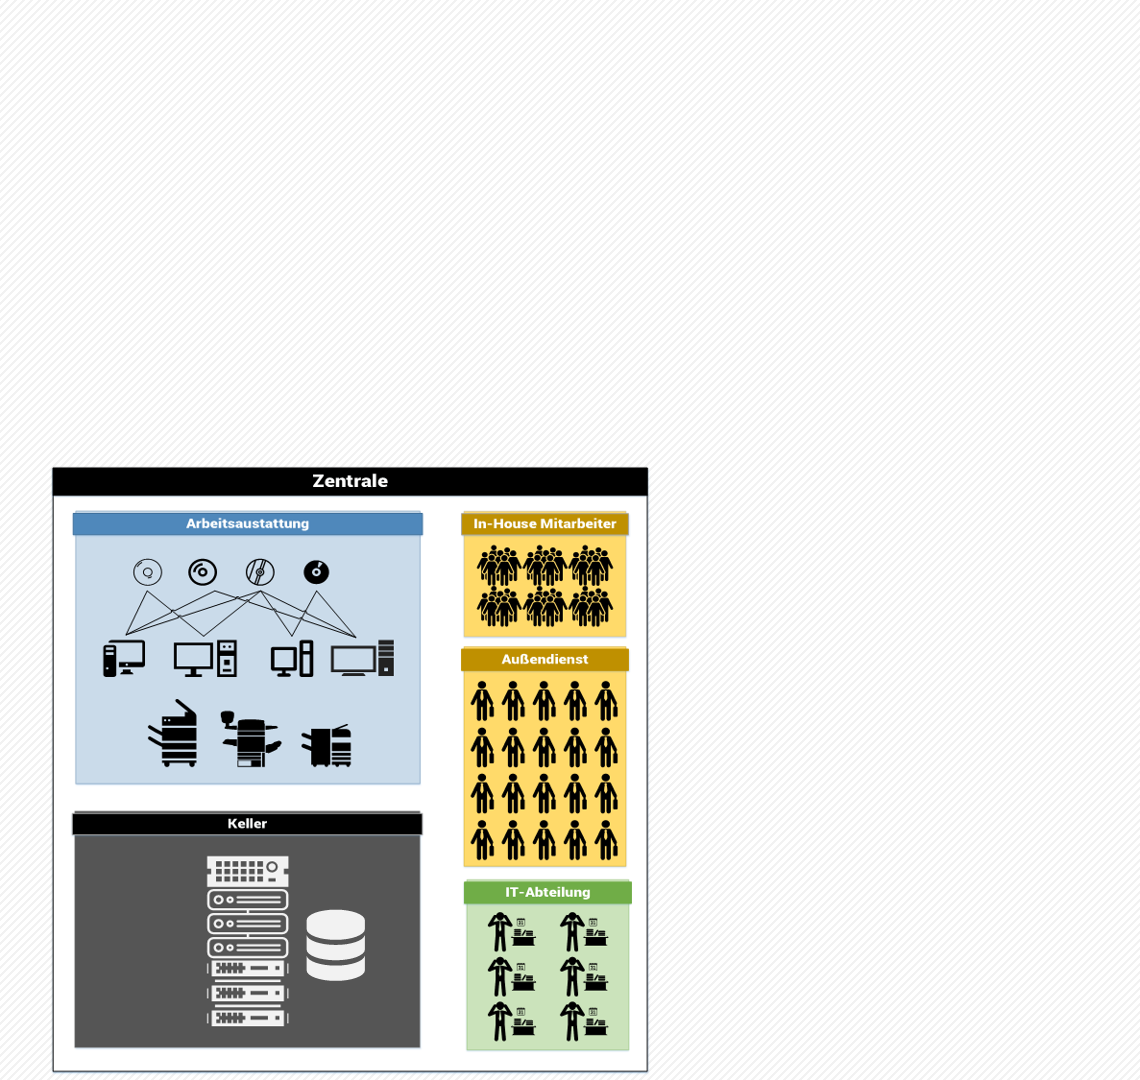
\includegraphics[width=1\textwidth]{img/Umbau1}}\\}
\caption{Ausgangssituation} % Überschrift
\source{Eigene Darstellung} % Quelle
\end{minipage}
\end{figure}

\textbf{\underline{Schritt 1:}}\\
Die Cloud wird eingerichtet (Auswahl und Bestellung beim Cloud-Anbieter, Einrichtung der Zugriffsverbindungen, Erstellung benötigter Partitionen, etc.).

Wenn noch nicht getan, soll nun die Abbildung des Unternehmen Stylez ins Multichannel-System geplant werden (Berechtigungskonzept, Abhängigkeiten, Organisationsmanagement, Geschäftsprozesse, etc.).
Dies soll mit Hilfe eines SAP-Partners geschehen, falls keine passenden Kompentenzen im Unternehmen vorhanden sind.
\begin{figure}[H]
\centering
\begin{minipage}[t]{0.9\textwidth}
{\centering\fbox{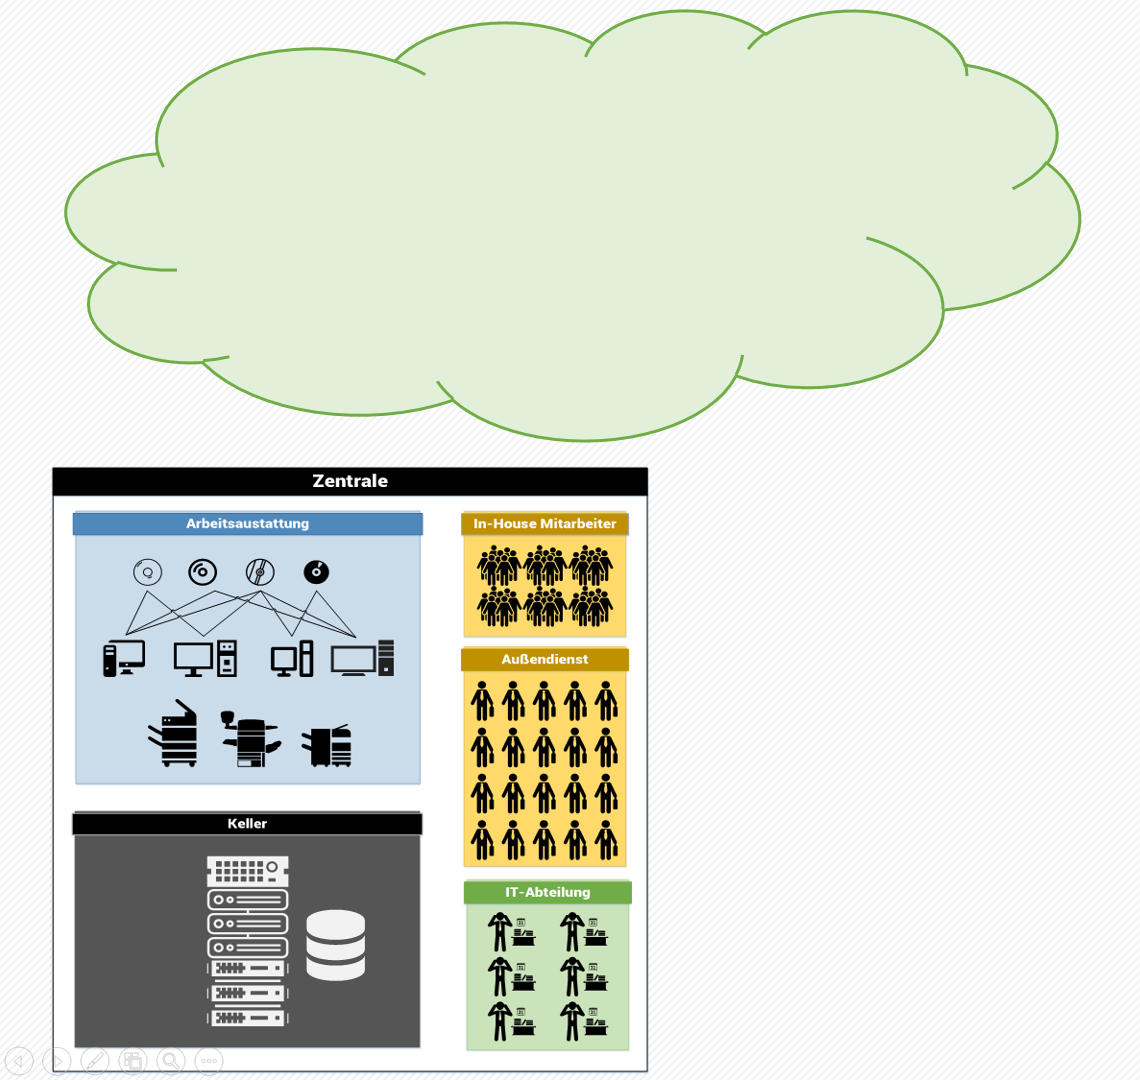
\includegraphics[width=1\textwidth]{img/Umbau2}}\\}
\caption{Schritt 1: Einrichtung der Clout} % Überschrift
\source{Eigene Darstellung} % Quelle
\end{minipage}
\end{figure}
\newpage

\textbf{\underline{Schritt 2:}}\\
Das Multichannel-System (Hybris, CRM, ERP, Solution Manager) wird in der Public Cloud installiert und nach der Planung aus Schritt 1 eingerichtet.\\
Nach der Einrichtung werden die Applikationsserver in der Unternehmenszentrale abgeschaltet, da sie nicht mehr benötigt werden. Die vorhandene Datenbank wird nun als Datenbasis für das Multichannel-System genutzt.

Da das Unternehmen Stylez ein kleines und übersichtliches Unternehmen ist, lässt sich dank Rapid Deployment Solution\footnote{Siehe auch Kapitel \ref{sec:RDS} auf Seite \pageref{sec:RDS}} innerhalb kurzer Zeit ein Multichannel-System aufbauen.
\begin{figure}[H]
\centering
\begin{minipage}[t]{0.9\textwidth}
{\centering\fbox{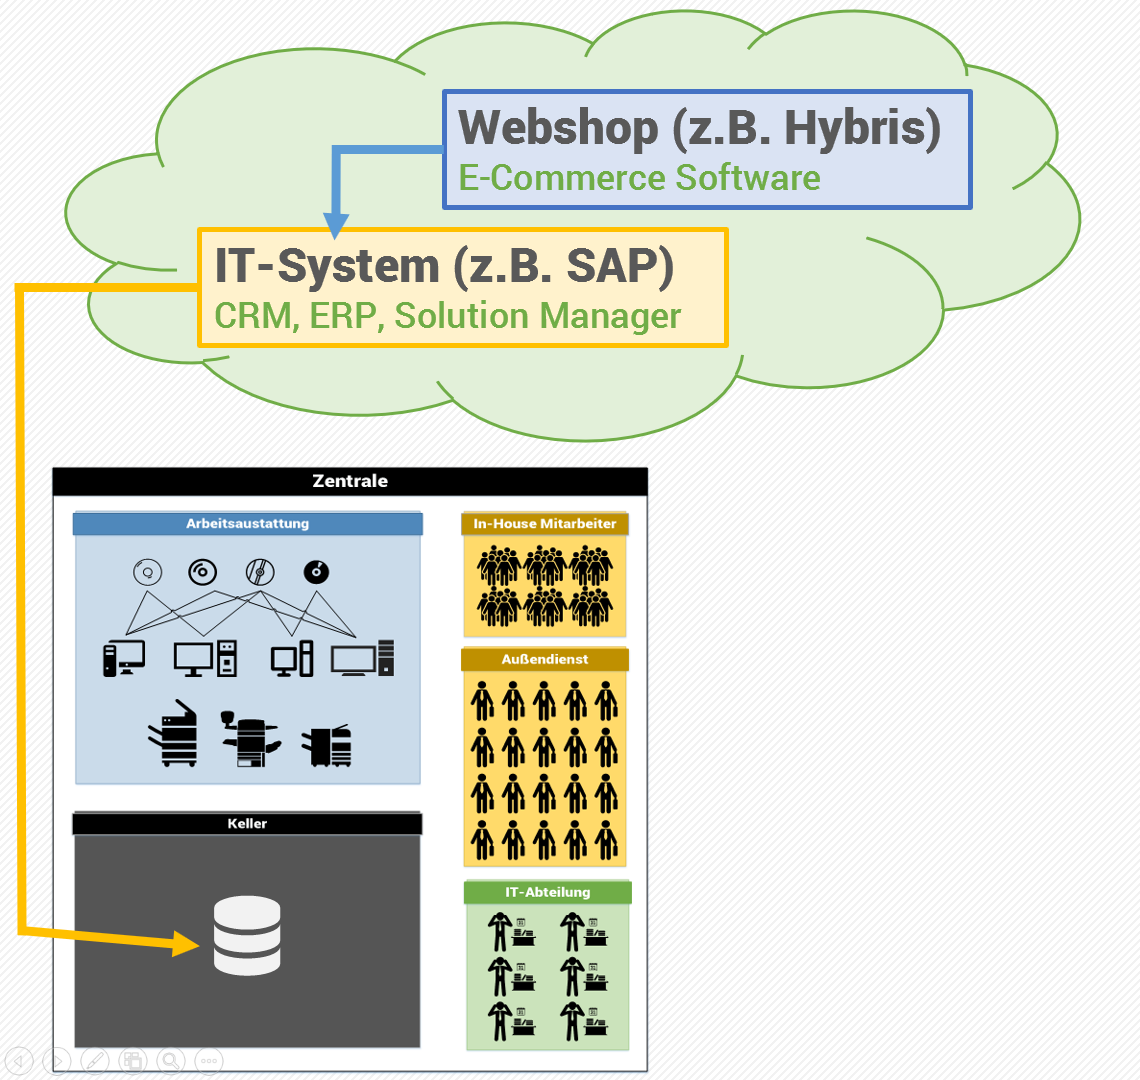
\includegraphics[width=1\textwidth]{img/Umbau4}}\\}
\caption{Schritt 2: Installation und Einrichtung der IT-Systeme in der Cloud} % Überschrift
\source{Eigene Darstellung} % Quelle
\end{minipage}
\end{figure}
\newpage

\textbf{\underline{Schritt 3:}}\\
Die Abbildung \ref{img:Multichannel_fertig} zeigt eine vereinfachte Darstellung des fertigen Multichannel-Systems.
\begin{figure}[H]
\centering
\begin{minipage}[t]{0.9\textwidth}
{\centering\fbox{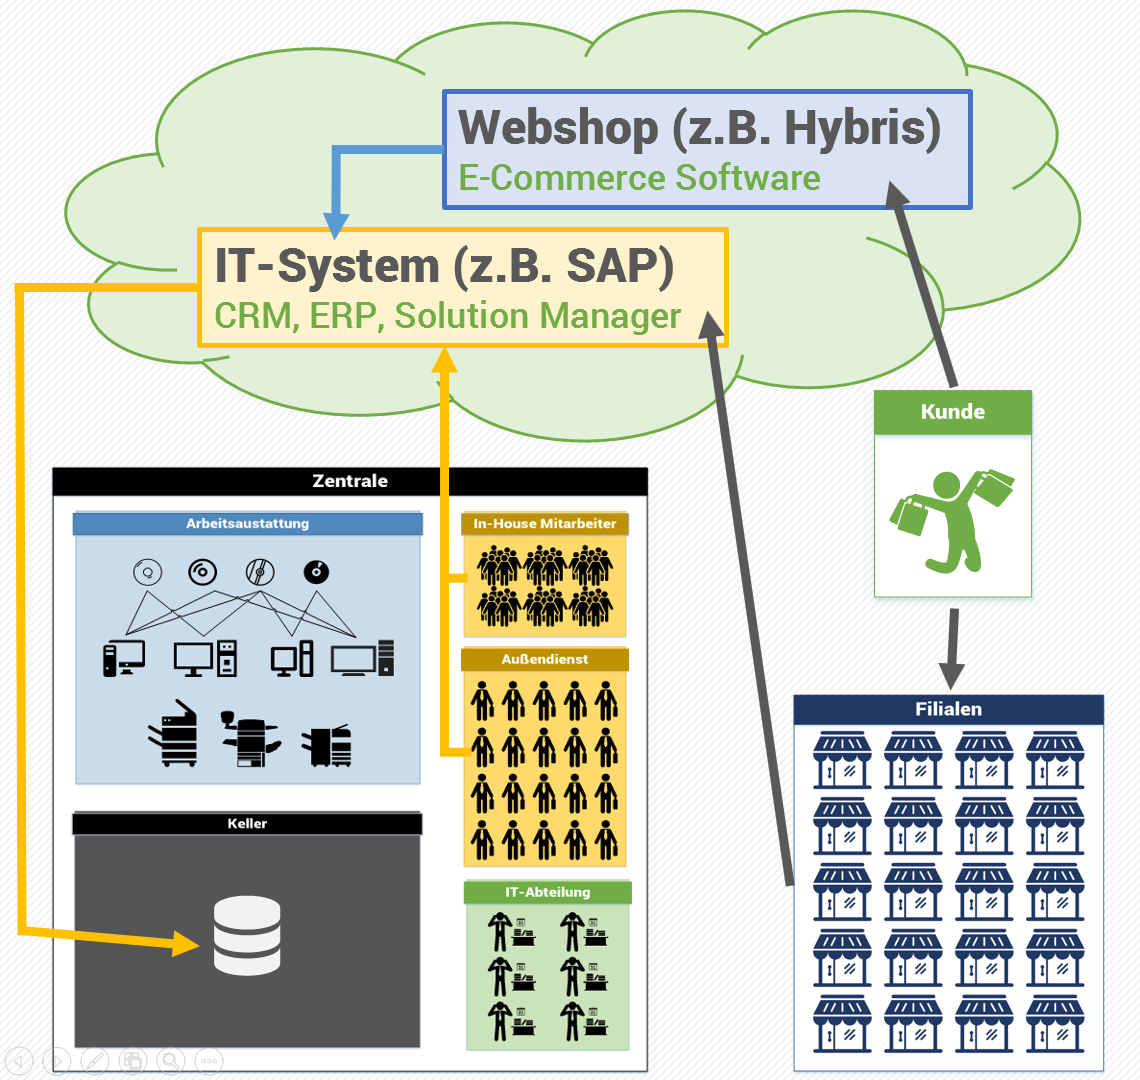
\includegraphics[width=1\textwidth]{img/Umbau5}}\\}
\caption{Schritt 3: Das fertige Multichannel-System} % Überschrift
\source{Eigene Darstellung} % Quelle
\label{img:Multichannel_fertig}
\end{minipage}
\end{figure}

Man kann sehen, dass das Multichannel-System die zentrale Anlaufstelle des Unternehmens ist und sehr stark bei der Verwaltung und Steuerung des Unternehmens hilft:
\begin{itemize}
\item Supportanfragen vom Außendienst, In-House Mitarbeitern und Franchisenehmern werden mit Hilfe des Help Desks im Solution Manager nach ITIL bearbeitet und per Dispatching an geeignete IT-Mitarbeiter weitergeleitet.
\item Die Filialen beziehen ihre IT-Leistungen und benötigten Daten vom ERP und CRM.
\item Kunden benutzen für das Online-Shopping (Stöbern, Informieren und Kaufen) den Hybris-Webshop.
\item Der Hybris-Webshop bezieht benötigte Informationen aus dem gesamten SAP-IT-System
\end{itemize}
Unabhängig von den Geschäftsprozessen wird die zentrale Datenbank, die wertvolle und vertrauliche Informationen enthält, nur von einer Komponente zugegriffen. Und zwar vom SAP-System.

Das bedeutet, dass bei richtiger Konfiguration durch den SAP-Partner und dem Cloud-Anbieter, nur Personen (oder Systemkomponenten), die ein SAP-Zugang besitzen und die notwendigen Berechtigungen haben, auf die empfindlichen Daten in der Datenbank zugreifen können. 

\subsection{Zusatz: SAP RDS (Rapid Deployment Solution)}
\label{sec:RDS}
\begin{figure}[H]
\centering
\begin{minipage}[t]{1\textwidth}
{\centering\fbox{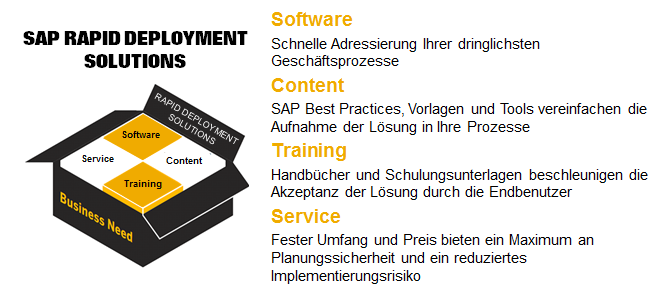
\includegraphics[width=1\textwidth]{img/RDS}}\\}
\caption{SAP RDS} % Überschrift
\source{https://wiki.scn.sap.com/wiki/display/CRM/SAP+CRM+Rapid+Deployment+Solutions,\\Stand: 21.04.2016} % Quelle
\end{minipage}
\end{figure}
Eine Einführung von SAP-Systemen wird aufgrund vieler Gründe wie z.B. großer Komplexität und hoher Risiken oft mit langen Projektphasen voller unerwarteter Fehler assoziiert. 
Mit RDS möchte SAP die Erwartungen und Anforderungen von IT-Abteilungen und Fachbereichen hinsichtlich Planungssicherheit und kurzer Implementierungszeit erfüllen:

\textit{\glqq SAP Rapid Deployment Solutions sind SAP-Lösungen, die zum Festpreis, mit klar definiertem Leistungsumfang und im Regelfall in höchstens 12 Wochen beim Kunden im Einsatz sein sollen. Die Lösungen kombinieren die bewährte SAP-Software mit Implementierungsservices von SAP Consulting oder SAP-Partnern, umfassen Best Practices, vorkonfigurierte Inhalte und Schulungsunterlagen für Endanwender.\grqq}\footcite[Online im Internet.]{RDS}

Da das Unternehmen Stylez klein und übersichtlich ist, ist die Abbildung des Unternehmens in das Multichannel-System nicht kompliziert und aufwändig. Und SAP bietet für ein Multichannel-System mit Hybris auch eine Rapid Deployment Solution an. Aus diesem Grund soll SAP im Unternehmen mit RDS eingeführt werden.

\section{Roadmap (An-Nam Pham)}
Die Roadmap dient als kurze Zusammenfassung aller Schritte für die Optimierung der IT als Zeitplan:
\begin{figure}[H]
\centering
\begin{minipage}[t]{1\textwidth}
{\centering\fbox{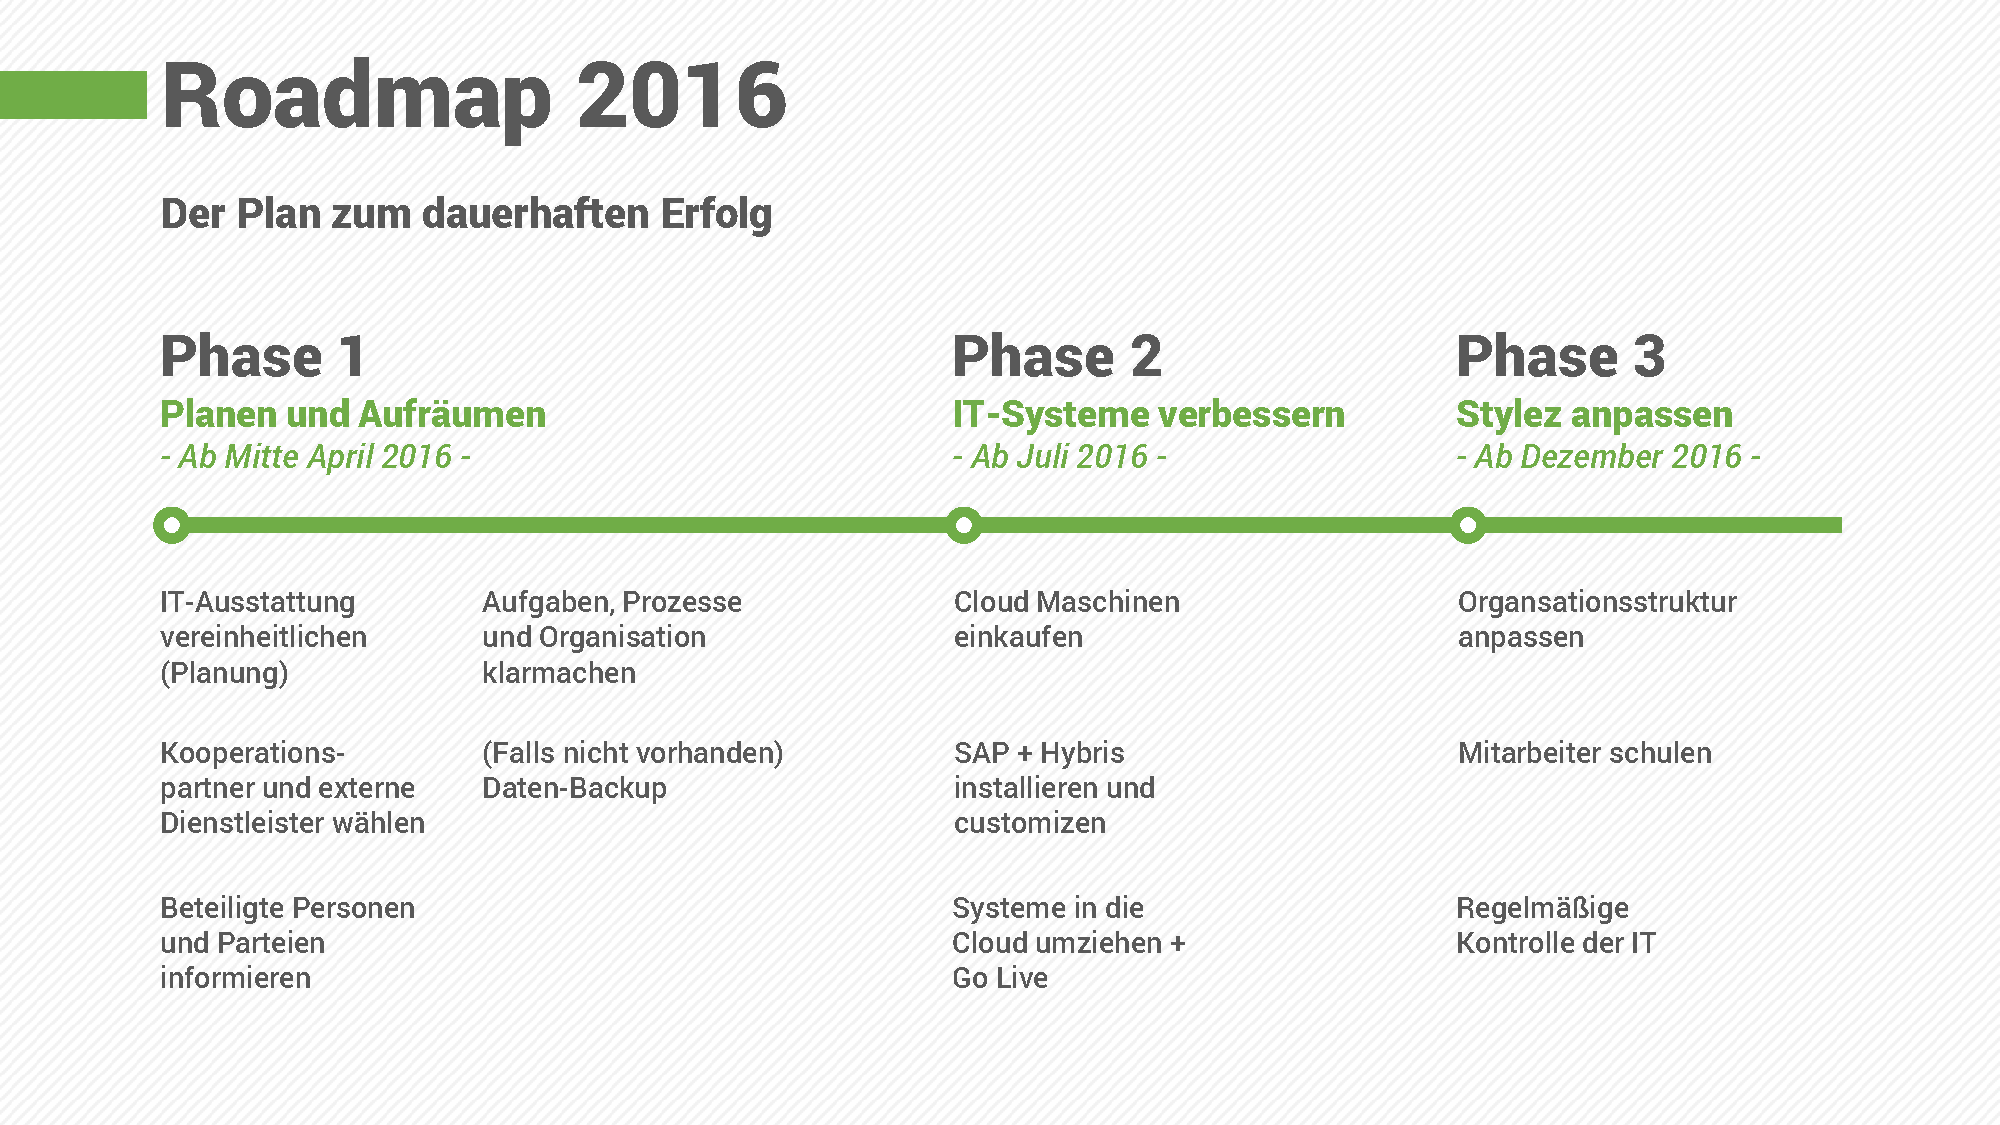
\includegraphics[width=1\textwidth]{img/Roadmap.pdf}}\\}
\caption{Die Roadmap 2016 für die IT-Optimierung bei Stylez} % Überschrift
\source{Eigene Darstellung} % Quelle
\label{img:Roadmap}
\end{minipage}
\end{figure}
% \section{Stichwort: Hochverfügbarkeit}
